\section{Method}
\begin{figure}[t]
    \centering
    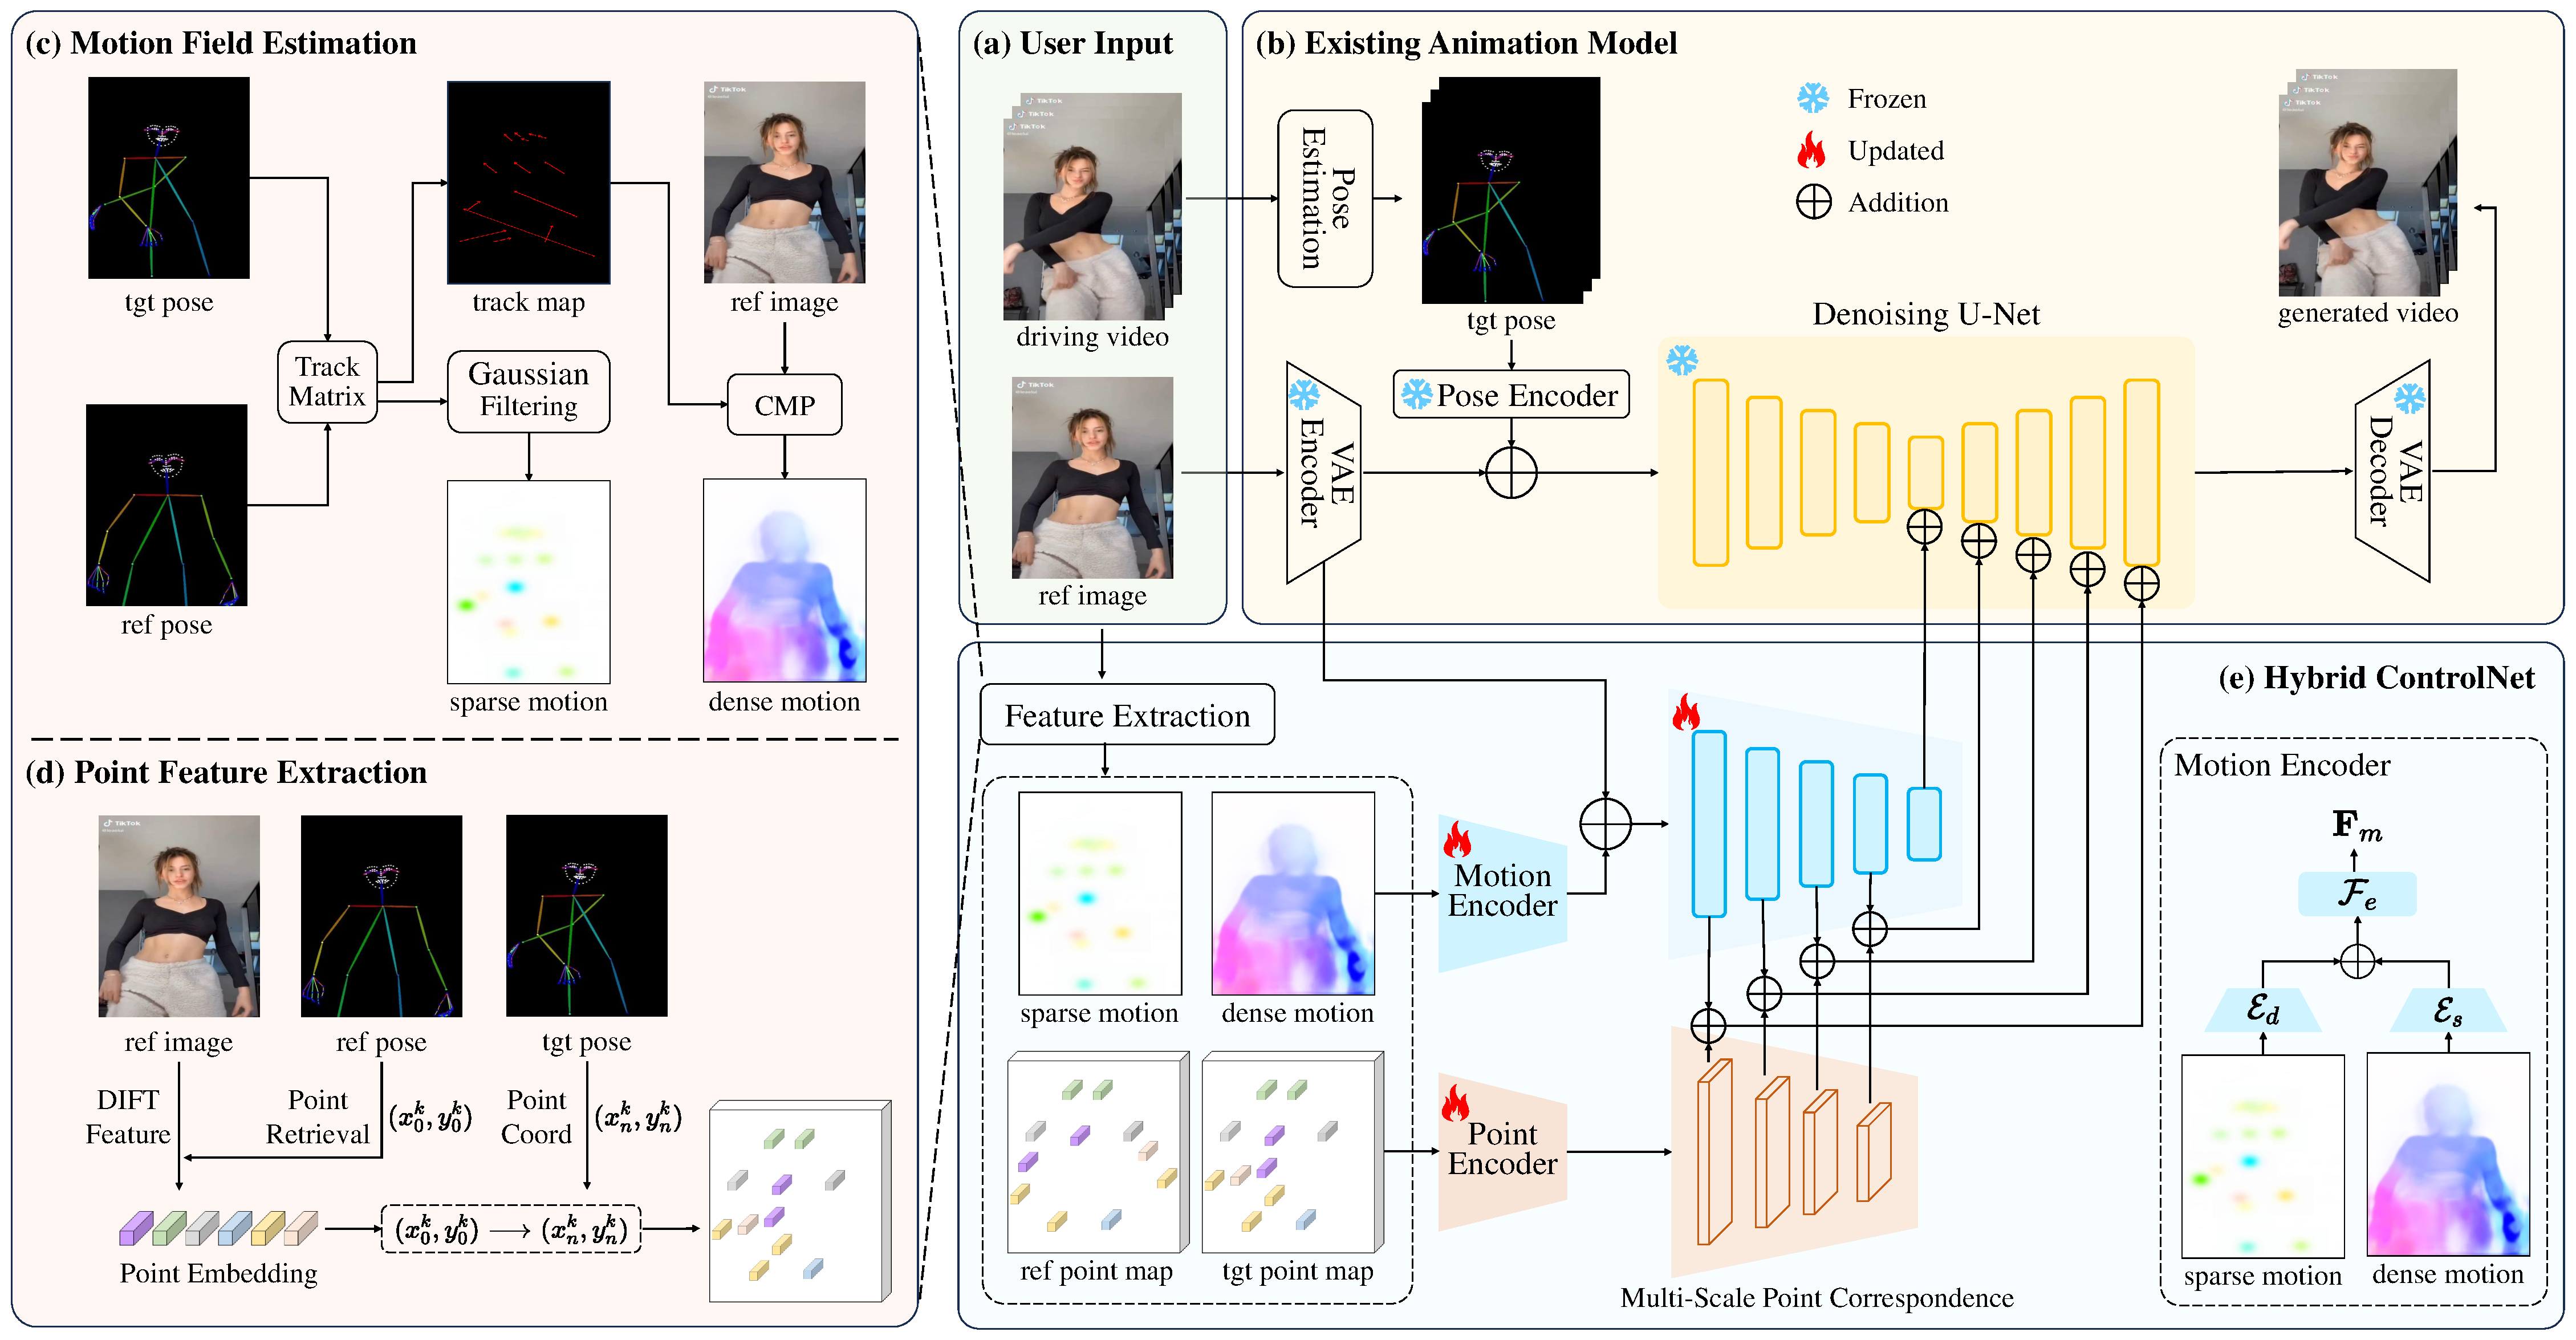
\includegraphics[width=1.0\columnwidth]{./image/pipeline.pdf}
    \vspace{-15pt}
    \caption{The overview of proposed DisPose.}
    \label{fig:pipeline}
\end{figure}
\section{DisPose}
Given a reference image $I_{\mathrm{ref}}\!\in\!\mathbb{R}^{3 \times H \times W}$ and a driving video $V\!\in\!\mathbb{R}^{N\times 3 \times H \times W}$. The core of our method is to disentangle efficient control guidance from only skeleton poses and reference images as shown in Figure~\ref{fig:pipeline}, which can be applied to existing human animation methods without additional dense inputs. We first introduce sparse and dense motion field guides in Sec.~\ref{sec: motion}. Then, we introduce reference-based keypoint correspondence in Sec.~\ref{sec: keypoint}. Finally, we introduce the pipeline of hybrid ControlNet in Sec~\ref{sec: controlnet}.
\subsection{Motion Field Guidance}
\label{sec: motion}

\textbf{Sparse Motion Field.}
We first estimate the skeleton pose by DWpose~\citep{yang2023dwpose} to obtain each frame's human key point coordinates. 
% Subsequently, the motion trajectory of all semantic points in the entire video is obtained and represented as
Subsequently, the key points of the reference image are used as starting points to track the motion displacement of all frames and represented as $P_{traj}\!=\!\{(x^k_n,y^k_n) \!\mid\! k=1\dots K, n=0\dots N\}$, where $P_{traj}$ denotes the trajectory map of the key point $k$ overall $N$ frames and $n = 0$ denotes the reference image. We calculate the track matrix $P_{s}$ as follows:
\begin{equation}
    \mathbf{P}_{s}=\{(x^k_n-x^k_{n-1}, y^k_n-y^k_{n-1}) \mid n=1\dots N\}\},
\end{equation}
% where $P_{t}$ denotes the trajectory map of the key point point $k$ over all $N$ frames, and the reference frame when $n = 0$.
where $K$ denotes the number of keypoints, $N$ denotes the number of frames, $\mathbf{P}_{s}$ denotes the trajectory map of keypoint k over all N frames, and $n = 0$ denotes the reference image.
To avoid training instability caused by overly sparse trajectory matrice, we then apply Gaussian filtering to enhance $\mathbf{P}_{s}$ to obtain the sparse motion field $\mathbf{F}_s\!\in\!\mathbb{R}^{(N-1)\times 2 \times H \times W}$ inspired by~\citep{yin2023dragnuwa, wang2024motionctrl}.

\textbf{Dense Motion Field.}
Considering that sparse control provides limited guidance and dense control is hard to obtain during inference,
% For the dense motion field, 
we transform dense guidance into the motion propagation from the reference frame to the target pose, instead of the dense signal of the target pose. Specifically, in the inference, we reconstruct the trajectory map $\mathbf{P}_{s}$ as the reference-based sparse optical flow $\mathbf{P}_{d}$ from the reference frame to each target pose as:
\begin{equation}
    \mathbf{P}_{d}=\{(x^k_n-x^k_{0}, y^k_n-y^k_{0}) \mid n=1\dots N\}\},
\end{equation}
We then predicted the reference-based dense motion filed $\mathbf{F}_d\!=\! \text{CMP}(P_{traj}, \mathbf{P}_{d}, I_{ref})\!\in\!\mathbb{R}^{(N-1)\times 2 \times H \times W}$ by condition motion propagation (CMP)~\citep{zhan2019self} based on the sparse optical flow $\mathbf{P}_{d}$ and the reference image $I_{ref}$.
CMP~\citep{zhan2019self} is a self-supervised learning-from-motion model that acquires an image and a sparse motion field and estimates the corresponding dense motion field.
Notably, the dense motion field $\mathbf{F}_d$ of each frame starts with the reference image, which avoids geometric constraints during inference.

To ensure motion estimation accuracy during training, we first extract the forward optical flow from the driving video using existing optical flow estimation models~\citep{teed2020raft, xu2023unifying}. We then use a watershed-based approach~\citep{zhan2019self} to sample the sparse optical flow $\mathbf{P}_{d}$ from the forward optical flow. See Appendix.~\ref{sec: appendix1} for details.

\textbf{Motion Encoder.} To leverage motion field as guidance, we introduce a motion encoder specifically designed for the optional flow, which includes sparse motion encoder $\mathcal{E}_s$, dense motion encoder $\mathcal{E}_d$ and feature fusion layer $\mathcal{F}_e$. $\mathcal{E}_d$ and $\mathcal{E}_s$ have the same structure and are multi-scale convolutional encoders with each stage built by \texttt{Conv-SiLU-ZeroConv}~\citep{zhang2023adding} as the basic block. The feature fusion layer $\mathcal{F}_e$ is a 2D convolution for fusing sparse motion features $\mathcal{E}_s(\mathbf{F}_s)$ and dense motion features $\mathcal{E}_d(\mathbf{F}_d)$. Finally, we compute the motion field guidance $\mathbf{F}_m$:
\begin{equation}
    \mathbf{F}_m = \mathcal{F}_e(\mathcal{E}_s(\mathbf{F}_s)+\mathcal{E}_d(\mathbf{F}_d))
\end{equation}

\subsection{Keypoint Correspondence}
\label{sec: keypoint}
\textbf{Point Feature Extraction.} 
To maintain a consistent appearance, it is crucial to correspond the content of the reference image with the motion trajectory. 
Specifically, we first extract the DIFT~\citep{tang2023emergent} features $\mathbf{D}$ of the reference image using the pre-trained image diffusion model. 

Subsequently, the keypoint embedding in the reference is obtained as $\mathbf{D}(x^k_0,y^k_0)$, where $(x^k_0,y^k_0)$ is retrieved from the reference pose.
% key point embeddings $\mathbf{D}(x^k_0,y^k_0)$ are retrieved from $\mathbf{D}$ by skeleton pose $(x^k_0, y^k_0)$.
Next, we initialize the keypoint correspondence map $\mathbf{F}_p$ with zero vectors and assign point embeddings according to the trajectory coordinates as:
\begin{equation}
\label{eq: v prob}
f^{ij}_n=\left\{\begin{array}{ll}
\mathbf{D}(x^k_0,y^k_0), & \mathrm{if} \quad i=x^k_n, j=y^k_n,  \\
0, & \mathrm{otherwise}.
\end{array}\right.
\end{equation}

Finally, we obtain the keypoint correspondence map $\mathbf{F}_p=\{f_n\!\mid\!n=1\dots N\} \!\in\!\mathbb{R}^{N\times D_p \times H \times W}$ for all frames, where $D_p$ is the feature dimension of the point embedding.

\textbf{Point Encoder.} 
To utilize the content correspondence of key points as guidance, we generate multi-scale correspondences of sparse point feature maps and make them compatible with the U-Net encoder of the {Hybrid ControlNet (Sec.4.3)}. 
% as detailed in F. 1.
We introduce the multi-scale point encoder $\mathcal{E}_p$ to maintain the key point content $\mathbf{F}_p$ from the reference image. The point encoder $\mathcal{E}_p$ consists of a series of learnable MLPs.
{
To seamlessly integrate into existing models, we extract intermediate features of the encoder of the hybrid Controlnet.
The multi-scale intermediate features of the Controlnet encoder are denoted as $\mathbf{E}^l_{enc}$, where $l$ denotes each U-Net block $l\!\in\![1, L]$.}
To match the spatial size of $\mathbf{E}^l_{enc}$, we apply downsampling to the feature map between the encoder layers. We compute the multi-scale keypoint correspondence as follows:
\begin{equation}
    \mathbf{F}_c^l = \mathcal{E}_p^l(\phi(\mathbf{F}_p, H^l, W^l)),
\end{equation}
where $(H^l, W^l)$ are denote the spatial dimension of the $l$-th U-Net block and $\phi$ means downsampling operation. Therefore, $\mathbf{F}_c^l$ shares the same size as $\mathbf{E}^l_{enc}$.
Finally, $\mathbf{F}_c$ are added elementwisely to the intermediate feature $\mathbf{E}^l_{enc}$ of the U-Net encoder as guidance: $\mathbf{E}^l_{enc}\!=\!\mathbf{E}^l_{enc}+\mathbf{F}_c^l$.


\subsection{Plug-and-play Hybrid ControlNet}
\label{sec: controlnet}
After obtaining motion field guidance and keypoint correspondence, we aim to integrate these control guidance seamlessly into the U-Net architecture of existing animation models.
Inspired by ControlNet~\citep{zhang2023adding}, We design a hybrid ControlNet $\mathcal{F}$ to provide additional control signals for the existing animation model as shown in Figure~\ref{fig:pipeline}(e).
% Specifically, we consider freeze denoising U-Net and pose encoder. 
Specifically, given an animation diffusion model based on the U-Net architecture, we freeze all its modules while allowing the motion encoder, point encoder and hybrid ControlNet to be updated during training. 
Subsequently, $\mathbf{F}_m$ is added to the noise latent before being input into the hybrid ControlNet. Considering the high sparsity of the point feature $\mathbf{F}_c$, we correspondingly add $\mathbf{F}_c$ to the input of the convolutional layer. Notably, the U-Net encoder intermediate feature $\mathbf{E}_{enc}$ in Sec.~\ref{sec: keypoint} is from hybrid ControlNet rather than denoising U-Net. Finally, 
the control condition is computed as:
\begin{equation}
    \boldsymbol{r}=\mathcal{F}(\boldsymbol{z}_{{t}} \mid \mathbf{F}_m, \mathbf{F}_c, {t})
\end{equation}
where $\boldsymbol{r}$ is a set of condition residuals added to the residuals for the middle and upsampling blocks in the denoising U-Net.

Given a monocular video containing camera motions, a moving human, and a static scene, our method automatically disentangles and represents the human and the static scene with 3D Gaussians.
%
The human Gaussians are initialized using the \smpl body model and the scene Gaussians are initialized from the structure-from-motion point cloud from COLMAP~\cite{colmapschoenberger2016mvs, colmapschoenberger2016sfm}.
%
In the following, we first quickly review 3D Gaussian splatting and the \smpl body model. Then, we introduce the proposed method to address challenges when modeling and animating humans in the 3D Gaussian framework.  

\subsection{Preliminaries}

\paragraph{3D Gaussian Splatting (3DGS)~\cite{kerbl3Dgaussians}}
%3D Gaussians are parameterized by means $\bm\mu$, rotation $\bm{R}$, and scale $\bm{S}$. 
%
represents a scene by arranging 3D Gaussians. 
%
The $i$-th Gaussian is defined as 
%
\begin{equation}
    G(\mathbf{p}) = o_i \, e^{-\frac{1}{2} (\mathbf{p} - \bm\mu_i)^T \bm\Sigma_{i}^{-1} (\mathbf{p} - \bm\mu_i)},
    \label{eq:gauss3d}
\end{equation}
%
where $\mathbf{p} \, {\in} \, \mathbb{R}^3$ is a xyz location, $o_i \, {\in} \, [0, 1]$ is the opacity modeling the ratio of radiance the Gaussian absorbs, $\bm\mu_i \, {\in} \, \mathbb{R}^3$ is the center/mean of the Gaussian, and the covariance matrix $\bm\Sigma_{i}$ is parameterized by the scale $\mathbf{S}_{i} \, {\in} \, \mathbb{R_+}^3$ along each of the three Gaussian axes and the rotation $\mathbf{R}_{i} \, {\in} \, SO(3)$ with $\bm\Sigma_{i} = \mathbf{R}_{i} \mathbf{S}_{i} \mathbf{S}_{i}^\top \mathbf{R}_{i}^\top$.
%
Each Gaussian is also paired with spherical harmonics~\cite{ramamoorthi2001efficient} to model the radiance emit towards various directions. 
% 
%
% The $i$-th 3D Gaussian is parameterized by its mean $\bm\mu_i \in \mathbb{R}^3$, scales along each dimension $\mathbf{S}_{i} \in \mathbb{R_+}^3$, and rotation $\mathbf{R}_{i}\in SO(3)$.
%
% The covariance matrix is calculated by $\bm\Sigma_{i} = \mathbf{R}_{i} \mathbf{S}_{i} \mathbf{S}_{i}^\top \mathbf{R}_{i}^\top$.
%
% Each Gaussian is also paired with an opacity $o_i \in [0, 1]$, to model the ratio of radiance it absorbs, and a 4th-degree spherical harmonics~\cite{ramamoorthi2001efficient}, to model the radiance it emits toward various directions. 
%
% A 3D Gaussian is parameterized by its mean $\bm\mu_i \in \mathbb{R}^3$ and its covariance matrix $\bm\Sigma_{i} \in $, which is parameterized by rotation $\mathbf{R}_{i}\in SO(3)$ and scales $\mathbf{S}_{i} \in \mathbb{R}^3$. 

% the $\bm\Sigma_{i}$ into a rotation component $\mathbf{R}_{i}\in SO(3)$ and a scale component $\mathbf{S}_{i} \in \mathbb{R}^3$ where $\bm\Sigma_{i} = \mathbf{R}_{i} \mathbf{S}_{i} \mathbf{S}_{i}^\top \mathbf{R}_{i}^\top$.
%
% Each gaussian represents a physical space, we can compute the influence of a Gaussian to a point $\mathbf{p} \in \mathbb{R}^3$ by evaluating the probability density function

% \begin{equation}
%     G(\mathbf{p}) = \sigma({o_i}) e^{-\frac{1}{2} (\mathbf{p} - \bm\mu_i)^T \bm\Sigma_{i}^{-1} (\mathbf{p} - \bm\mu_i)},
%     \label{eq:gauss3d}
% \end{equation}
%
%where $o_i \in \mathbb{R}$ is the opacity of each gaussian and $\sigma$ is the sigmoid function. The view-dependent appearance of individual Gaussians is represented with 4th-degree spherical harmonics~\cite{ramamoorthi2001efficient}.

% represents an area of 3D physical space which is occupied by solid matter with a probability density function. %
% Each Gaussian influences a point in physical 3D space $p \in \mathbb{R}^3$ weighted by its opacity $o_i \in \mathbb{R}$ according to the standard (unnormalized) Gaussian equation,
% \begin{equation}
% f_{i}(p) = \sigma({o_i}) \exp\left( -\frac{1}{2} (p - \mu_{i})^T \Sigma_{i}^{-1} (p - \mu_{i}) \right),
% \label{eq:gauss3d}
% \end{equation}

% where ${\mu}_{i} \in \mathbb{R}^3$
% % = \begin{bmatrix} x_{i} &  y_{i} &  z_{i} \end{bmatrix}^T$ 
% is the center, and $\Sigma_{i} = R_{i} S_i S_i^T R_{i}^T$ is the covariance matrix of Gaussian $i$, with the scaling component $S_i \in \mathbb{R}^3 $ 
% %= \text{diag}\left(\begin{bmatrix} sx_i & sy_i & sz_i \end{bmatrix}\right)$,
% and the rotation component $R_{i} \in SO(3)$,
% %= \textrm{q2R}\left(\begin{bmatrix} qw_{i} & qx_{i} & qy_{i} & qz_{i} \end{bmatrix}\right)$, where $\textrm{q2R}()$ is the formula for constructing a rotation matrix from a quaternion. 
% and $\sigma$ is the standard sigmoid function.

% Each Gaussian's influence $f$ is both inherently local (being able to represent a small area of space), while also theoretically having infinite extent, such that gradients can flow to them even from a long distance, which is crucial for gradient-based differentiable rendering that optimizes for the position of 3D Gaussians. The softness of the 3D Gaussian representation also means that Gaussians typically need to significantly overlap in order to represent a physically solid object. As well as physical density, each Gaussian contributes its own appearance to each of the 3D points it influences.


During rendering, the 3D Gaussians are projected onto the image plane and form 2D Gaussians~\cite{zwicker2001surface} with the covariance matrix $\bm\Sigma_{i}^{\textrm{2D}} = \bm{J} \bm{W} \bm\Sigma_{i} \bm{W}^\top \bm{J}^\top$,
%following Zwicker \etal~\cite{zwicker2001surface} 
%
% \begin{equation}
%     \bm\Sigma_{i}^{\textrm{2D}} = J W \bm\Sigma_{i} W^\top J^\top,
% \end{equation}
%
where $\bm{J}$ is the Jacobian of the affine approximation of the projective transformation and $\bm{W}$ is the viewing transformation. 
% to We splat 3D Gaussians on the image plane by approximating the projection of the integral of $G$ function along the depth dimension of the 3D Gaussian into a 2D Gaussian influence function in pixel coordinates. The center of the Gaussian is splatted using the standard point rendering formula,
% $$\mu^{\textrm{2D}} = K \left((E \mu) / (E \mu)_z\right)$$
% where the 3D Gaussian center $\mu$ is projected into a 2D image by multiplication with the world-to-camera extrinsic matrix $E$, z-normalization, and multiplication by the intrinsic projection matrix $K$. The 3D covariance matrix is splatted into 2D using the formula from \cite{zwicker2001surface}:
% $$\Sigma^{\textrm{2D}} = J E \Sigma E^T J^T$$
% where $J$ is the Jacobian of the point projection formula above, i.e. $\partial \mu^{\textrm{2D}} / \partial \mu$.
%
The color of a pixel is calculated via alpha blending the $N$ Gaussians contributing to a given pixel: 
%
\begin{equation}
    C = \sum_{j = 1}^{N} c_j \alpha_{j} \prod_{k=1}^{j-1} (1 - \alpha_{k}),
\end{equation}
%
where the Gaussians are sorted from close to far, $c_j$ is the color obtained by evaluating the spherical harmonics given viewing transform $W$, and $\alpha_j$ is calculated from the 2D Gaussian formulation (with the covariance $\bm\Sigma_{j}^{2D}$) multiplied by its opacity $o_j$.
%
The rendering process is differentiable, which we take advantage of to learn our human model.

% The influence function $f$ can now be evaluated in 2D for each pixel for each Gaussian. The influence of all Gaussians on this pixel can be combined by sorting the Gaussians in depth order and performing front-to-back volume rendering using the volume rendering formula (the same as is used in NeRF \cite{mildenhall2020nerf}):
% $$C_{\text{pix}} = \sum_{i \in \mathcal{S}} c_i f^{\textrm{2D}}_{i, \textrm{pix}} \prod_{j=1}^{i-1} (1 - f^{\textrm{2D}}_{j, \textrm{pix}})$$
% where the final rendered color ($C_{\text{pix}}$) for each pixel is a weighted sum over the colors of each Gaussian ($c_i = \begin{bmatrix} r_i &  g_i &  b_i \end{bmatrix}^T$), weighted by the Gaussian's influence on that pixel $f^{\textrm{2D}}_{i, \textrm{pix}}$ (the equivalent of the formula for $f_i$ in 3D except with the 3D means and covariance matrices replaced with the 2D splatted versions), and down-weighted by an occlusion (transmittance) term taking into account the effect of all Gaussians in front of the current Gaussian. 

% \ar{Move this $\downarrow$ to implementation section}
% We use the CUDA implementation by Kerbl \etal~\cite{kerbl3Dgaussians} which enables fast training and rendering speeds $\sim$50 FPS for 1080p images.
%
%
% The implementation of \cite{kerbl20233d} uses a number of graphics and CUDA optimization techniques to achieve fast rendering speeds (\eg, $50$ FPS for our scenes), which therefore also enables very fast training.


\paragraph{SMPL~\cite{SMPL:2015}} is a parametric human body model which allows pose and shape control. 
%
The \smpl model comes with a template human mesh $(\template, \bm{F})$ in the rest pose (\ie, T-pose) in the template coordinate space. 
%
$\template \, {\in} \, \mathbb{R}^{\numverts \times 3}$ are the $\numverts$ vertices on the mesh, and $\bm{F} \, {\in} \, \mathbb{N}^{\numfaces\times 3}$ are the $\numfaces$ triangles with a fixed topology. 
%
Given the body shape parameters, $\shapecoeff \, {\in} \, \shapespaceexpl$, and the pose parameters, $\posecoeff \, {\in} \, \posespaceexpl$, \smpl transforms the vertices $\template$ from the template coordinate space to the shaped space via
%
\begin{equation}
    T_S(\shapecoeff, \posecoeff) = \template + B_{S}(\shapecoeff) +  B_{P}(\posecoeff),
    \label{eq:smpl vertex}
\end{equation}
%
where $T_S(\shapecoeff, \posecoeff)$ are the vertex locations in the shaped space, $B_{S}(\shapecoeff) \, \in \, \mathbb{R}^{\numverts \times 3}$ and $B_{S}(\posecoeff) \, \in \, \mathbb{R}^{\numverts \times 3}$ are the xyz offsets to individual vertices.
%
The mesh in the shaped space fits the identity (\eg, body type) of the human shape in the rest pose. 
%
%The mesh contains $\numverts$ vertices $\bm{V}\in\mathbb{R}^{\numverts\times 3}$ and $\numfaces$ triangles $\bm{F}\in\mathbb{R}^{\numfaces\times 3}$ with a fixed topology. 
%
To animate the human mesh to a certain pose (\ie, transforming the mesh to the posed space), \smpl utilizes $\numjoints$ predefined joints and Linear Blend Skinning (LBS).
%
The LBS weights $\bm{W} \, {\in} \, \mathbb{R}^{\numjoints {\times} \numverts}$ are provided by the \smpl model.
%
Given the $i$-th vertex location on the resting human mesh, $\bm{p}_i \, {\in} \, \mathbb{R}^3$, and individual posed joints' configuration (\ie, their rotation and translation in the world coordinate), $\bm{G} = [\bm{G}_1, \dots, \bm{G}_{\numjoints}]$, where $\bm{G}_k \, {\in} \, SE(3)$, the posed vertex location $\bm{v}_i$ is calculated as $\bm{v}_i = \left( \sum_{k=1}^{n_k} W_{k,i} \, \bm{G}_k \right) \bm{p}_i$, 
%
% \begin{equation}
% \small
% \begin{aligned}
%     \underbrace{\bm{v}_i}_{\textnormal{Posed vertex}} = \underbrace{\sum_{k=1}^{n_k}\bm{W}_{k,i} \, G_k }_{\textnormal{Transformation to the posed space}} {\bm{p}_i},
% \end{aligned}
% \end{equation}
%
where $W_{k,i} \, {\in} \, \mathbb{R}$ is the element in $\bm{W}$ corresponding to the $k$-th joint and the $i$-th vertex. 
%
While the \smpl model provides an animatable human body mesh, it does not model hair and clothing. 
%
Our method utilizes \smpl mesh and LBS only during the initialization phase and allows Gaussians to deviate from the human mesh to model details like hairs and clothing. 
%
% Our method only uses \smpl to initialize the human Gaussians, allowing the Gaussians to capture those details.
%
% To capture more geometric details, we use an upsampled version of \smpl with $\numverts \, {=} \, 110,210$ vertices and $\numfaces \, {=} \, 220,416$ faces.


\subsection{Human Gaussian Splats}

Given $T$ captured images and their camera poses, we first use a pretrained \smpl regressor~\cite{goel2023humans4d} to estimate the \smpl pose parameters for each image, $\bm{\theta}_1, \dots, \bm{\theta}_T$, and the body shape parameters, $\bm\beta$, that is shared across images.\footnote{We also obtain a coordinate transformation from \smpl's posed space to the world coordinate (used by the camera poses) for each frame, following Jiang \etal~\cite{jiang2022neuman}. For simplicity, we will ignore the coordinate transformation in the discussions.} 
%
Our method represents the human with 3D Gaussians and drive the Gaussians using a learned LBS. 
%
Our method outputs the Gaussian locations, rotations, scales, spherical harmonics coefficients, and their LBS weights with respect to the $\numjoints$ joints. 
%
% We also jointly optimize a different set of Gaussians representing the static scene. 
%
% \jg{This sentence needs to be clearer. Tie back to our intro about how separation of the human is a feature. Or is this "therefore in this method we focus on the human part"}The static scene is modeled using the standard 3DGS, and thus we focus on introducing the Human Gaussians. 
%
An overview of our method is illustrated in \cref{fig:overview}. 


The human Gaussians are constructed from their center locations in a canonical space, a feature triplane~\cite{Peng2020ECCV,Chan2022} $\bm{F} \, {\in} \, \mathbb{R}^{3{\times}h{\times}w{\times}d}$, and three Multi-Layer Perceptrons (MLPs) which predict properties of the Gaussians.
%
All of them are optimized per person.
%
The Human Gaussians live in a canonical space, which is a posed space of \smpl where the human mesh performs a predefined Da-pose.
%


\paragraph{Rendering process.} Given a joint configuration $\bm G$, to render an image, for each Gaussian, we first interpolate the triplane at its center location $\bm{\mu}_i$ and get feature vectors $\bm{f}_x^i, \bm{f}_y^i, \bm{f}_z^i \, {\in} \, \mathbb{R}^d$.
%
The feature $\bm{f}^i$ representing the $i$-th Gaussians is the concatenation of $\bm{f}_x^i, \bm{f}_y^i, \bm{f}_z^i$.
%
Taking $\bm{f}^i$ as input, an appearance MLP, $D_A$, outputs the RGB color and the opacity of the $i$-th Gaussian; a geometry MLP, $D_G$, outputs an offset to the center location, $\Delta \bm{\mu}_i$, the rotation matrix $\bm{R}_i$ (parameterized by the first two columns), and the scale of three axes $\bm{S}_i$; a deformation MLP, $D_D$, outputs the LBS weights, $\bm{W}_i \, {\in} \, \mathbb{R}^{\numjoints}$ for this Gaussian.
%
The LBS uses $\bm{W}$ and the joint transformation $\bm G$ to transform the Human Gaussians, which are then combined with the Scene Gaussians and splat onto the image plane.
%
The rendering process is end-to-end differentiable. 


\paragraph{Optimization.} We optimize the center locations of the Gaussians $\bm{\mu}$, the feature triplane, and the parameters of the three MLPs.\footnote{We also follow Jiang \etal~\cite{jiang2022neuman} and adjust the per image \smpl pose parameters $\bm{\theta}$ during the optimization, since $\bm{\theta}$ are initialized by an off-the-shelf \smpl regressor~\cite{goel2023humans4d} and may contain errors (see the details in the supplementary material).}
%
The rendered image is compared with the ground-truth captured image using $\mathcal{L}_1$ loss, the SSIM loss~\cite{ssim} $\mathcal{L}_{\text{ssim}}$, and the perceptual loss~\cite{simonyan2015vgg} $\mathcal{L}_{\text{vgg}}$. 
%\ot{citation for lvgg}
%
We also render a human-only image (using only the human Gaussians on a random solid background) and compare regions containing the human in the ground-truth image using the above losses.
%
The human regions are obtained using a pretrained segmentation model~\cite{kirillov2023segmentanything}. 
%
We also regularize the learned LBS weights $\bm{W}$ to be close to those from SMPL with an $\ell_2$ loss.
%
Specifically, to regularize the LBS weights $\bm{W}$, for individual Gaussians we retrieve their $k=6$ nearest vertices on the \smpl mesh and take a distance-weighted average of their LBS weights to get $\hat{\bm{W}}$. The loss is $\mathcal{L}_{\text{LBS}} = \| \bm{W} - \hat{\bm{W}} \|_{\text{F}}^2$.

%
% We use the same losses to optimize the scene Gaussians jointly.
%
Specifically, our loss is composed of
\begin{multline}
\mathcal{L} = \underbrace{\lambda_1 \mathcal{L}_1 + \lambda_2 \mathcal{L}_{\text{ssim}} + \lambda_3 \mathcal{L}_{\text{vgg}}}_{\text{scene + human}} \\ + \underbrace{\lambda_1 \mathcal{L}^h_1 + \lambda_2 \mathcal{L}^h_{\text{ssim}} + \lambda_3 \mathcal{L}^h_{\text{vgg}}}_{\text{human}} + \lambda_4 \mathcal{L}_{\text{LBS}},
\end{multline}
%
where $\lambda_1 = 0.8$, $\lambda_2 = 0.2$, $\lambda_3 = 1.0$, $\lambda_4 = 1000$ for all scenes in the experiments.
%
We employ the Adam optimizer~\cite{KingBa15} with a learning rate of $10^{-3}$, coupled with a cosine learning rate schedule.




%
We initialize the center of the Gaussians, $\bm\mu$, at the canonical-posed \smpl mesh vertices (so we have the same number of Gaussians as the \smpl vertices at the beginning of the optimization). We pretrain the feature triplane and the MLPs to output RGB color as $[0.5, 0.5, 0.5]$, opacity $o = 0.1$, $\Delta \bm{\mu} = 0$, rotation $\bm{R}$ so that z-axis of the Gaussians align with the corresponding \smpl vertex normal, scale $\bm{S}$ as the average incoming edges' lengths, and LBS weights $\bm{W}$ as those from \smpl (since the Gaussians lie exactly on the \smpl vertices).
%
The pretraining takes 5000 iterations (1 minute on a  GeForce 3090Ti GPU).
%
We use an upsampled version of \smpl with $\numverts \, {=} \, 110,210$ vertices and $\numfaces \, {=} \, 220,416$ faces.
%
Note that the \smpl mesh and LBS weights are only used in the initialization and regularization, \ie, they are not used during testing.


During the optimization, similar to the standard 3DGS, we clone, split, and prune Gaussians, every 600 iterations, based on their loss gradient and opacity.
%
They are important steps to avoid local minima during the optimization.
%
To clone and split, we simply add additional entries in $\bm{\mu}$ by repeating existing centers (cloning) and randomly sampling within the Gaussians with respect to their current shapes (\ie, $\bm{R}$ and $\bm{S}$) (splitting).
%
To prune a Gaussian, we remove it from $\bm{\mu}$.
%
Since the new Gaussians' centers are close to the original ones on the triplane, their features are similar and thus the new Gaussians have similar shape as the originals, allowing the optimization to proceed normally.
%
To make the split Gaussians smaller, we record a base scale $s \in \mathbb{R}_+$ for each Gaussian. The base scale is initialized as 1 and every time a Gaussian is split, we divide the base scale by 1.6. The actual scale of the Gaussian is $s$ multiplied with the MLP estimate $\bm{S}$.
%
The entire optimization takes 12K iterations, and 30 minutes on a GeForce 3090Ti GPU.  At the end of the optimization, the human is represented by 200K Gaussians on average.
%

\paragraph{Test-time rendering.} Importantly, after the optimization, the 3D Gaussians can be explicitly constructed, allowing direct animation of the human Gaussians using the LBS weights.
%
In other words, we \textit{do not need to evaluate} the triplane and MLPs to render new human poses. 
%
This is a big advantage compared to methods that represent human as implicit neural fields.


% \ot{We should mention that, after we learn the model we convert the representation to explicit therefore we do not need to evaluate the NNs during rendering new poses. This is a big adventage.}

% \ar{More details.., splitting the gaussians, mlp architecture in supp mat?}

% In order to model a human body using 3DGS, we start from 3D points on a template mesh of a human body and treat them as a 3D Gaussians. 
% %Our main idea is to start from Gaussians initialized from SMPL template and learn the
% We learn the geometry, appearance, and deformation over the set of Gaussians on the template. To this end, we represent the human in canonical space using the SMPL template $\template$ which is subdivided to $\numverts$ vertices. Each vertex is associated by a 3D Gaussian modeled using Eq.~\ref{eq:gauss3d}. The gaussian means $\bm\mu_i$ are initialized from SMPL vertices directly. We initialize the Gaussian rotations $\bm{R}_i$  using the SMPL vertex normals. For scale $\bm{S}_i$ initialization, we compute the mean of edge lengths $l_{edge}$ for a given mesh vertex and set $\bm{S}_i = [l_{edge}, l_{edge}, 10^{-4}]$. Following the Kerbl \etal~\cite{kerbl3Dgaussians} opacity $o_i$ is initialized as $0.1$. 

% \ar{need to switch the GCN part}
% In order to model the personalized geometry, clothing, and deformation details, we use graph convolutional network (GCN)-based modules that operates on the surface of our Gaussian mesh and the surface triangulation of the template mesh $(\mu, R, S, F)$. Our model uses three graph convolutional decoder networks -- a geometry decoder $D_G$ that models geometric offsets in the canonical space, an appearance decoder $D_A$, and a deformation decoder $D_D$. The input to these decoder networks is learnable Gaussian embeddings $G_{embed} \in \mathbb{R}^{72}$. The network $D_G$ predicts the deformation of the Gaussian mean $\Delta \bm\mu$, rotation $\Delta \bm{R}$ and scales $\Delta \bm{S}$ in the canonical space. The appearance network $D_A$ predicts the opacity $o_i$ and the spherical harmonics coefficients which is converted to $c_i$ following Ramamoorthi et al.~\cite{ramamoorthi2001efficient} for each of the Gaussians. Finally, the deformation network $D_D$ estimates pose-correctives~\cite{SMPL:2015} $B_P$ and the weights $W$ of the linear blend skinning function. The deformation of the Gaussians from canonical space to the observation is then given by,

% % \begin{align}
% %     \bm{T}_{G} &=  {\sum_{k=1}^{n_k}\bm{W}_{k,i}G_k(\bm{\theta},J(\bm{\beta}))} \\
% %     {\bm{\mu}_i^o} &= \bm{T}_{G} \cdot (\bm\mu_i + \Delta \bm\mu_i) \\
% %     {\bm{R}_i^o &= \bm{T}_{G} \cdot (\bm{R}_i \cdot \Delta \bm{R}_i)}
% % \end{align}

% \begin{align*} 
%     \bm{T}_{G} &= \sum_{k=1}^{n_k}\bm{W}_{k,i}G_k(\bm{\theta},J(\bm{\beta})) \\
%     \bm{\mu}_i^o &= \bm{T}_{G} \cdot (\bm\mu_i + \Delta \bm\mu_i) \\
%     \bm{R}_i^o &= \bm{T}_{G} \cdot (\bm{R}_i \cdot \Delta \bm{R}_i)
% \end{align*}

% where $\bm{T}_G$ is the global transformation matrix obtained by linearly blending the SMPL joint transformations. Here LBS weights $\bm W$ and pose-correctives $\bm{B}_P$ are estimated by deformation decoder $D_D$. $\bm{\mu}_i^o$ and $\bm{R}_i^o$ denote the deformed Gaussian parameters.

% \paragraph{Splitting the Gaussians}
% \ar{TBA}


% \subsection{Problems to deforming 3D Gaussians}

% \rick{we need to highlight the problems of using 3D gaussians to model/animate humans. In other words, we need to show why it is not a simple A+B method. It allows us to emphasize our contributions on pose-dependent deformation correction, GCN, and regularizations.  Please consider adding a figure to showcase with and without the addons.}

% \textcolor{red}{mention spherical harmonics rotation}

% \paragraph{GCN.}
% In order to human body deformation, we use a graph convolutional network (GCN) that operates on the surface of our gaussian mesh parametrizes by Gaussian means and the surface triangulation of the template mesh $(\mu, R, S, F)$. Our model uses three graph convolutional decoder networks -- a geometry decoder $D_G$ that models geometric offsets in the canonical space, an appearance decoder $D_A$, and a deformation decoder $D_D$. The network $G$ predicts the deformation of the Gaussian mean $\Delta \mu$, rotation $\Delta R$ and scales $\Delta S$ in the canonical space. The appearance network predicts the opacity $o_i$ Spherical Harmonics coefficients ... such that $c_i = SH_basis (\bm{n})$ following Ramamoorthi et al.~\cite{ramamoorthi2001efficient} for each of the Gaussians.  Finally, the deformation network $D_D$ pose-correctives~\cite{SMPL:2015} $B_P$ and the weights $W$ of the linear blend skinning function. The deformation of the Gaussians from canonical space to the observation is then given by,

% \begin{equation}
%     {\bm{\mu}_i^o} = {\sum_{k=1}^{n_k}\bm{W}_{k,i}G_k(\bm{\theta},J(\bm{\beta}))\cdot
%         \begin{bmatrix}
%      \bm{I} &  \bm{o}_i+ \bm{b}_i \\
%       \bm{0} &  1 
%   \end{bmatrix}}\cdot{\mu_i + \Delta \mu_i},
% \end{equation}


% \subsection{Joint Human-Scene Optimization}


% \paragraph{Initialization.}
% We use COLMAP~\cite{colmapschoenberger2016mvs, colmapschoenberger2016sfm} structure-from-motion to get camera parameters and a sparse scene point cloud. We use an off-the-shelf \smpl regressor~\cite{which_regressor} to obtain \smpl pose parameters $\posecoeff$ for each frame and the shared shape parameters $\shapecoeff$. Since the estimated $\posecoeff$ are not accurate, we optimize them using 2D joints estimated from \cite{xu2022vitpose} as detailed in the supplementary material. We then align the SMPL posed space to the world coordinate with a per-frame coodinate transformation, following Jiang \etal~\cite{jiang2022neuman}.

% \paragraph{Optimization.}
% We optimize the scene and human avatar jointly. We observed that joint optimization helps to alleviate the floating Gaussian artifacts for the scene and get sharper boundaries for the human model ~\ar{which we will discuss in \S 4.X?/suppmat}. Following Kerbl ~\etal~\cite{kerbl3Dgaussians} we use the adaptive control of Gaussians to get a denser set that better represents the scene. Please refer to Section 5.2 of \cite{kerbl3Dgaussians} for more details.

% During optimization, we employ image-based rendering losses together with human-specific regularizations during training. 

% \begin{equation}
%     \mathcal{L} = \mathcal{L}_1 + \mathcal{L}_{ssim} + \mathcal{L}_{vgg} + \mathcal{L}_{proj} + \mathcal{L}_{rep}
% \end{equation}

% Here $\mathcal{L}_1$ is the $\mathcal{L}_1$ loss between the rendered and ground-truth image, $\mathcal{L}_{ssim}$ is the $\mathcal{L}_{ssim}$ loss between the rendered and ground-truth image, and $\mathcal{L}_{vgg}$ is the perceptual loss between the rendered and ground-truth image. We use two regularizer losses on the human Gaussians $\mathcal{L}_{proj}$ and $\mathcal{L}_{rep}$. $\mathcal{L}_{proj}$ essentially enforces the Gaussian means to be $\bm{\mu}$ close to the local tangent plane of neighboring points by computing the PCA in a local neighborhood. \ar{$\mathcal{L}_{proj} equation?$}
% $\mathcal{L}_{rep}$ enforces Gaussians to be close to each other in a local neighborhood. \ar{$\mathcal{L}_{rep}$ equation?} We have $\lambda$ coefficients for each loss term presented here, but we removed them from the equation for brevity.

% Finally, we use Adam optimizer with learning rate $10^{-3}$ for decoder networks and $G_{embed}$ with a cosine learning rate scheduling~\cite{}.




% 3D Gaussian splatting is recently proposed by Kerbl \etal~\cite{kerbl3Dgaussians}. 

% We follow the \gstd~\cite{kerbl3Dgaussians} pipeline which is summarized below. Different from \gstd, we represent the humans in canonical space with \gauss We add a -- human deformation module (?) and .. ... , to improve .. .. .
% Our \gauss are defined by a full 3D covariance matrix $\Sigma$ defined in world space centered at point (mean) $\mu$:

% Following \cite{kerbl3Dgaussians}, the image formation model is given by
% \begin{equation}
%     C = \sum_{i \in N} c_i \alpha_i \prod_{j=1}^{i-1} 1 - \alpha_j
% \end{equation}
% where $C$ is the accumulated color at a pixel by blending $N$ points that overlap the pixel; and $\alpha_i$ is a function of opacity per point and the covariance of the 